\chapter{\uppercase{Xen Hypervisor}}

Xen is an open-source hypervisor, which started as a project at University of Cambridge. It uses paravirtualization in conjunction with hardware assisted virtualization technologies to develop a VMM. Along with widespread adoption, it also boasts of native support from Linux kernel.

\section{Xen Architecture}

Xen hypervisor follows a minimalist design policy with emphasis on security and efficiency. This is extremely important as the hypervisor hosts multiple Virtual Machines and any bugs could compromise the entire system. Virtual machines are hosted on custom environments called domains. Xen exposes very basic functionalities to these domains having similar UNIX counterparts as shown in Table ~\ref{tab:unixcomp}. Guest OSes should contain relevant modifications to use these features. 


\begin{figure}[H]
\centering
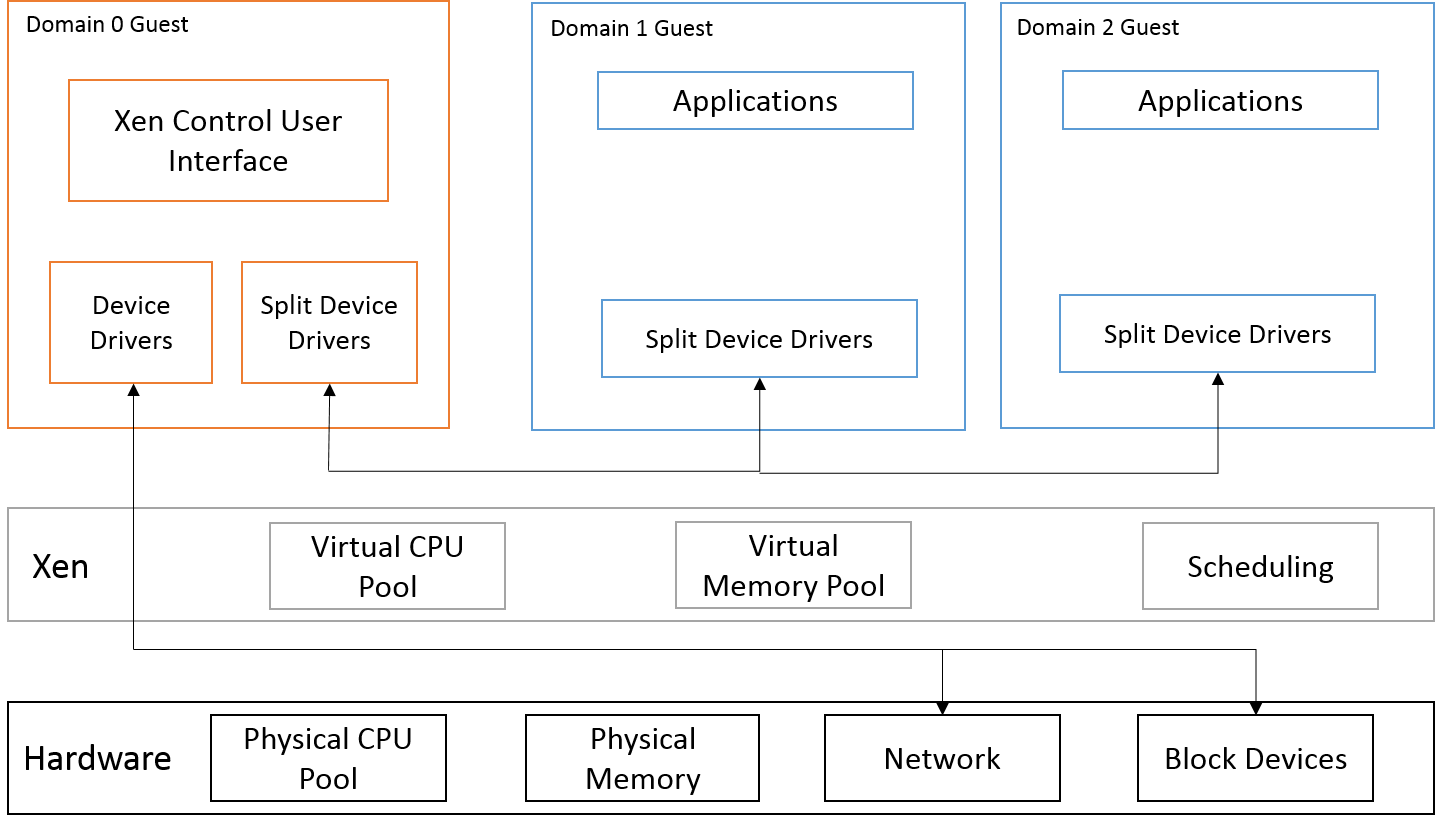
\includegraphics[scale=0.6]{figures/Xen_model.png}
\caption{Xen Architecture}
\label{tab:unixcomp}
\end{figure}
Initially Xen was designed for only paravirtualization on x86, i.e. Guest OS kernels were modified to be compatible with Xen. However, with the addition of Intel VT-x and AMD SVM extensions to the x86 architecture, it is possible to support pure virtualization. Guests on newer machines can run in two modes -- PV guest, or HVM Guest. In HVM mode Xen can run guests without any source code modifications. On the other hand, running a paravirtualized guest kernel in HVM takes the hybrid approach where the guest can take advantage of hardware features (such as Nested Page Tables), in addition to the performance boosts provided by paravirtualization techniques (such as hypercalls). Guests can use the CPUID instruction to prod whether it is running directly on hardware, or on top of Xen.  

 

The trap and emulate model, for hypervisors, is very expensive in terms of CPU cycles. Thus sensitive operations in a guest OS are typically replaced with hypercalls. This is quite similar to system calls in UNIX. Typically system calls use interrupt 80h (or SYSENTER instruction) to transfer control to the kernel in ring 0 with arguments either placed on the stack or in ISA registers. Hypercalls work in much the same way utilizing interrupt 82h instead in PV mode. However, in HVM mode, most interrupts are generally configured to be fed to the guest kernel instead of Xen. To enter the hypervisor at ring -1, a special instruction, VMCALL, is used instead. 

 

These two separate methods are unified in newer Xen versions via calling an address at a certain offset in a special page mapped to the Guest OS's address space. The offset determines the specific hypercall command. In the above method, the hypercall issue procedure remains the same from the Guest OS kernel's perspective whether in PV mode or in HVM mode. The implementation specifics are hidden in the page mapped to the Guest VM. 

 
In a Xen based system (Fig ~\ref{fig:xen_model}), memory and CPU resources are managed directly by the hypervisor, but I/O devices are generally controlled using a privileged domain (generally dom0 or Domain 0).Domain0. This domain runs in a higher privilege level where it is given significant access to most hardware resources. In addition to handling I/O operations, it also hosts the Xen User Interface used for administrative tasks. Thus, its security is of prime importance. Some of its responsibilities, such as hosting a device driver, can be delegated to domU guests (Guest domain) running at a higher privilege level. In certain cases of buggy device drivers, it is very useful, as during any device driver related fault, only the specific domU needs to be restarted instead of the entire system. However, in the absence of IOMMU, DMA requests from this domain can potentially affect memory regions allocated to other VMs. 

\begin{figure}[H]
\centering
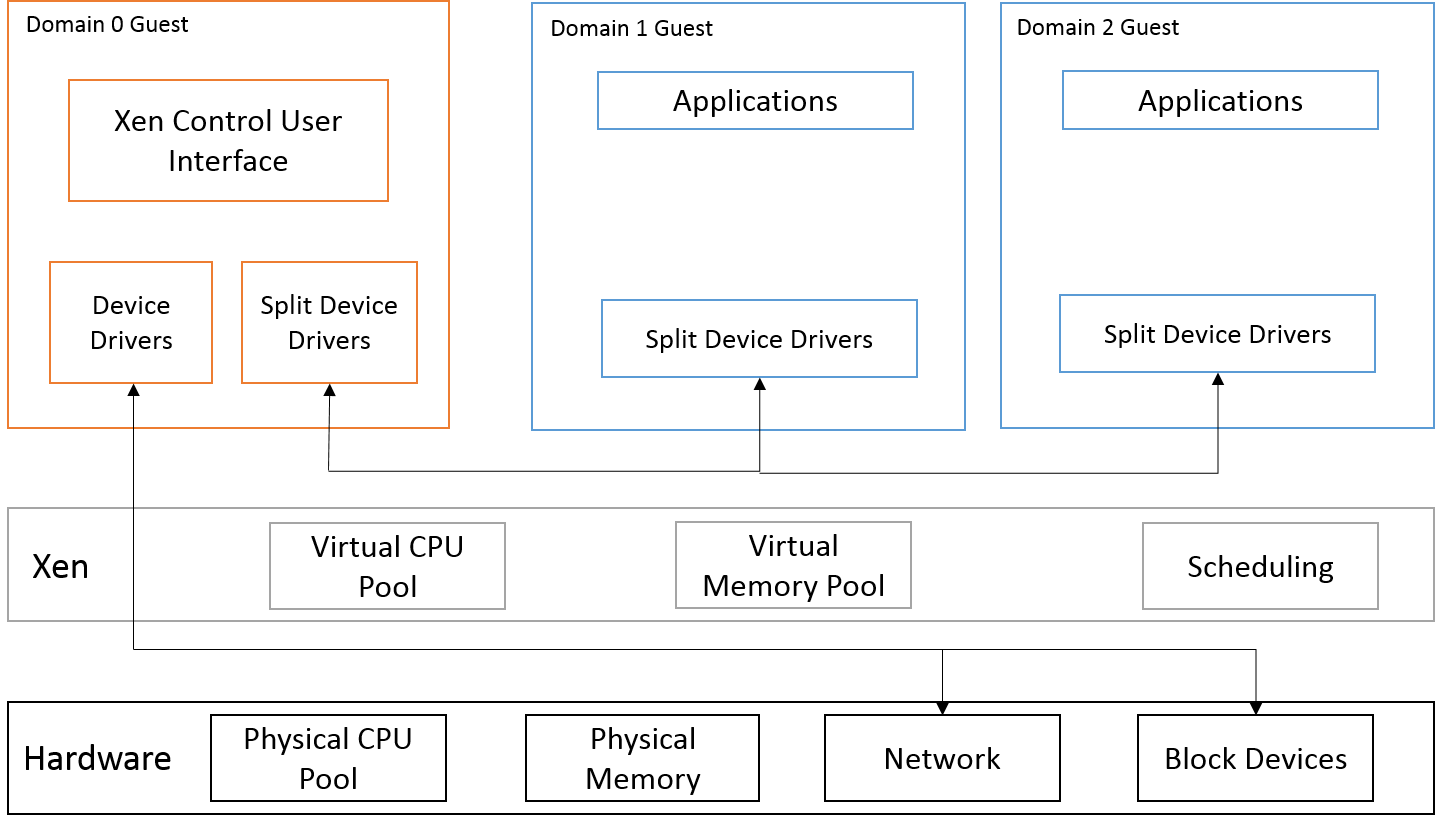
\includegraphics[scale=0.6]{figures/Xen_model.png}
\caption{Xen Architecture}
\label{fig:xen_model}
\end{figure}

Memory sharing in Xen is enabled via Grant tables. Memory is shared or transferred among domains at page granularity. This feature is quite useful in many situations such as networking among guests and implementing split device driver model. 

One of the features of Xen which makes it very popular is its I/O interface. Xen escapes the need to both emulate devices and develop separate device drivers with a split device driver model. It is made up of the following. 

1. Actual device driver. 

2. Generic backend driver. 

3. Generic frontend driver. 

4. Ring buffer. 

Typically, dom0 or a driver domain hosts the actual device drivers eliminating a notable amount of redundant developmental work. A generic frontend device driver is implemented in the guest domain at a much higher abstraction level which communicates with the backend device driver using ring buffers. The backend driver deconstructs the I/O requests from the front end driver and forwards it to the actual device driver. The requests are thus kept very simple avoiding device specific details. Ring buffers handle data movement across domains using shared memory utilities provided by Xen (Grant tables).  A key advantage of this model is that a single split device driver can cover a whole class of devices. 

Time keeping is another important aspect of an Operating System, especially for a scheduler. CPUs are shared amongst the running processes on a time sharing basis, and thus it is of utmost importance that the Operating System has accurate CPU clock information. Additionally, several userspace applications also need wall clock time information, which can be directly calculated from system time. Usually the above is gathered using the CPU clock and network time information. However, in a virtual machines the CPU clock does not reflect the system time, because different Operating Systems now share the same CPU. An additional issue now, is the difference between wall time and system time. This is where paravirtualization is quite useful, because the OS has to recognize the distinction between the two. Xen hypervisor holds the responsibility to provide a virtual machine with system time corresponding to the actual time the VM occupies a CPU. In HVM domains, Xen receives support from the hardware extensions, while in PV domain the above is performed entirely in software. 

\section{Xen Control Interface}
The control interface of Xen contains a combination of userspace, and kernel space code, through which hypercalls are issued. To host the interface, dom0 must comprise of a compliant kernel (Linux, NetBSD, Solaris, etc.) containing requisite modifications. The stack including and above Xend daemon, depicted in the figure below run as userspace space applications, while the rest run at a higher privilege level. 


\begin{figure}[H]
\centering
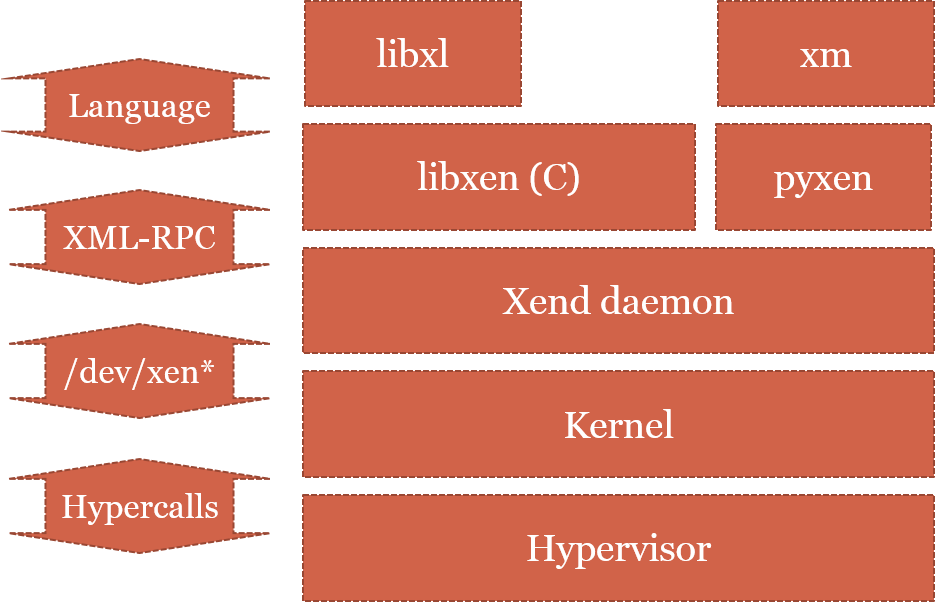
\includegraphics[scale=0.6]{figures/XEN_API.png}
\caption{Xen API}
\label{fig:xen_api}
\end{figure}

Xen commands issued through any tool, are converted to XML-RPC messages to communicate with the Xend daemon. Xend performs certain managerial tasks and either performs the relevant task itself, or forwards the command to the kernel to issue hypercalls. In this chain of flow, the interface of Xend daemon is standardized through the definition of Xen API. This allows development and proliferation of userspace management tools independent of changes lower in the stack. The complete Xen Control Interface structure is presented in Fig ~\ref{fig:xen_api}. Xen commands can be issued through a variety of userspace tools such as xl, xm, libvirt, etc. Some tools (e.g. xm) written in python, have an additional overhead of a runtime python environment. In contrast, xl is relatively lightweight using libxen library, written in C, to generate XML-RPC messages. 

The xend daemon runs in the userspace, thus minimizing dependence on a specific kernel. On receiving messages, xend performs certain critical tasks such as access control and issues hypercalls to the hypervisor through the kernel. 

 

Sample commands for xl toolchain are illustrated below: 

Create or start a virtual machine:  xl create <config\_filename> 

Shutdown a virtual machine:  xl shutdown <domain\_id> 


\section{Xen Memory Model}

Memory management is one of the core components of a hypervisor. With Xen core, the available memory is shared dynamically amongst the different virtual machines. It also allows for thin provisioning, i.e., projecting more memory than the available system RAM using ballooning techniques. 

 

As a part of design philosophy, Xen does not swap pages out of memory itself. Individual guest OSes’ are the best judges to identify cold pages and thus this job is left over to them. Using the balloon driver, Xen is able to mount or release memory pressure in a VM. When the hypervisor wants to reclaim pages from a VM, it inflates the balloon driver in the virtual machine. The balloon driver requests more memory from the OS, which swaps cold pages out and releases memory to the balloon driver. The latter in turn, returns those freed up memory pages to the hypervisor which can be allocated to the appropriate VM. During runtime, as the memory requirement is released, Xen deflates the balloon and releases memory back to the VM. The balloon driver monitors a target memory value, set in Xenstore to dynamically balance the actual memory allocated to the guest. This target memory value (set through domain0) is usually smaller than the guest physical address space and reflects the intended actual memory allocation for that domain. 

 

\subsection{x86\_64 Memory management}

This subsection focusses on the memory management details for x86\_64 machines. While extending the x86 ISA to 64 bits, AMD cleaned up memory segmentation controls, leaving a continuous flat address space with page level controls. In x86\_64, virtual memory is 64 bits wide, currently allowing only 48 bit sign extended addresses.  A typical system looks similar to Fig ~\ref{fig:x86_memspace}, having 128TB + 128TB accessible regions. 

\begin{figure}[H]
\centering
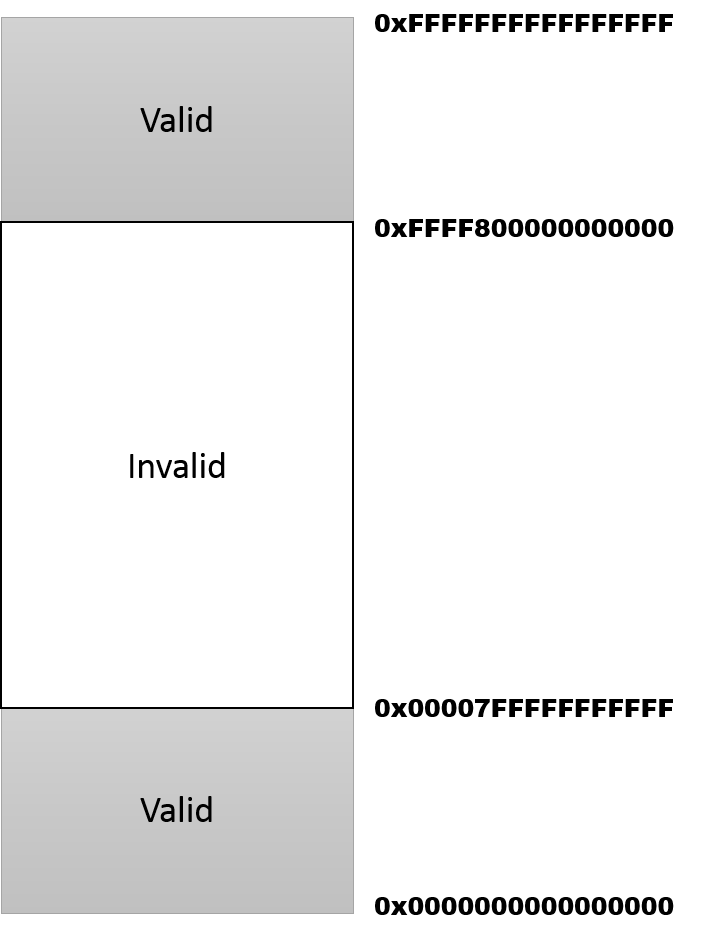
\includegraphics[scale=0.6]{figures/x86_64_VA_space.png}
\caption{x86\_64 Virtual Address Space}
\label{fig:x86_memspace}
\end{figure}

Typically for most Operating Systems, a virtual address space is generally divided into two parts 

1. Kernel Space: This space is shared and common to all the applications. Kernel space also contains a direct mapping of the physical address space (usually with an offset). 

2. Application Space: This space is specific to individual applications for application data and code. 

For Linux on x86\_64 machines, the lower region goes to the application and the upper region is occupied by the kernel. Mapping the kernel into the individual application address spaces avoids the overhead of a context switch during a system call. Moreover, many system calls pass arguments via a pointer to a userspace memory region, which is also accessible directly by the kernel, since the kernel is a part 


\begin{figure}[H]
\centering
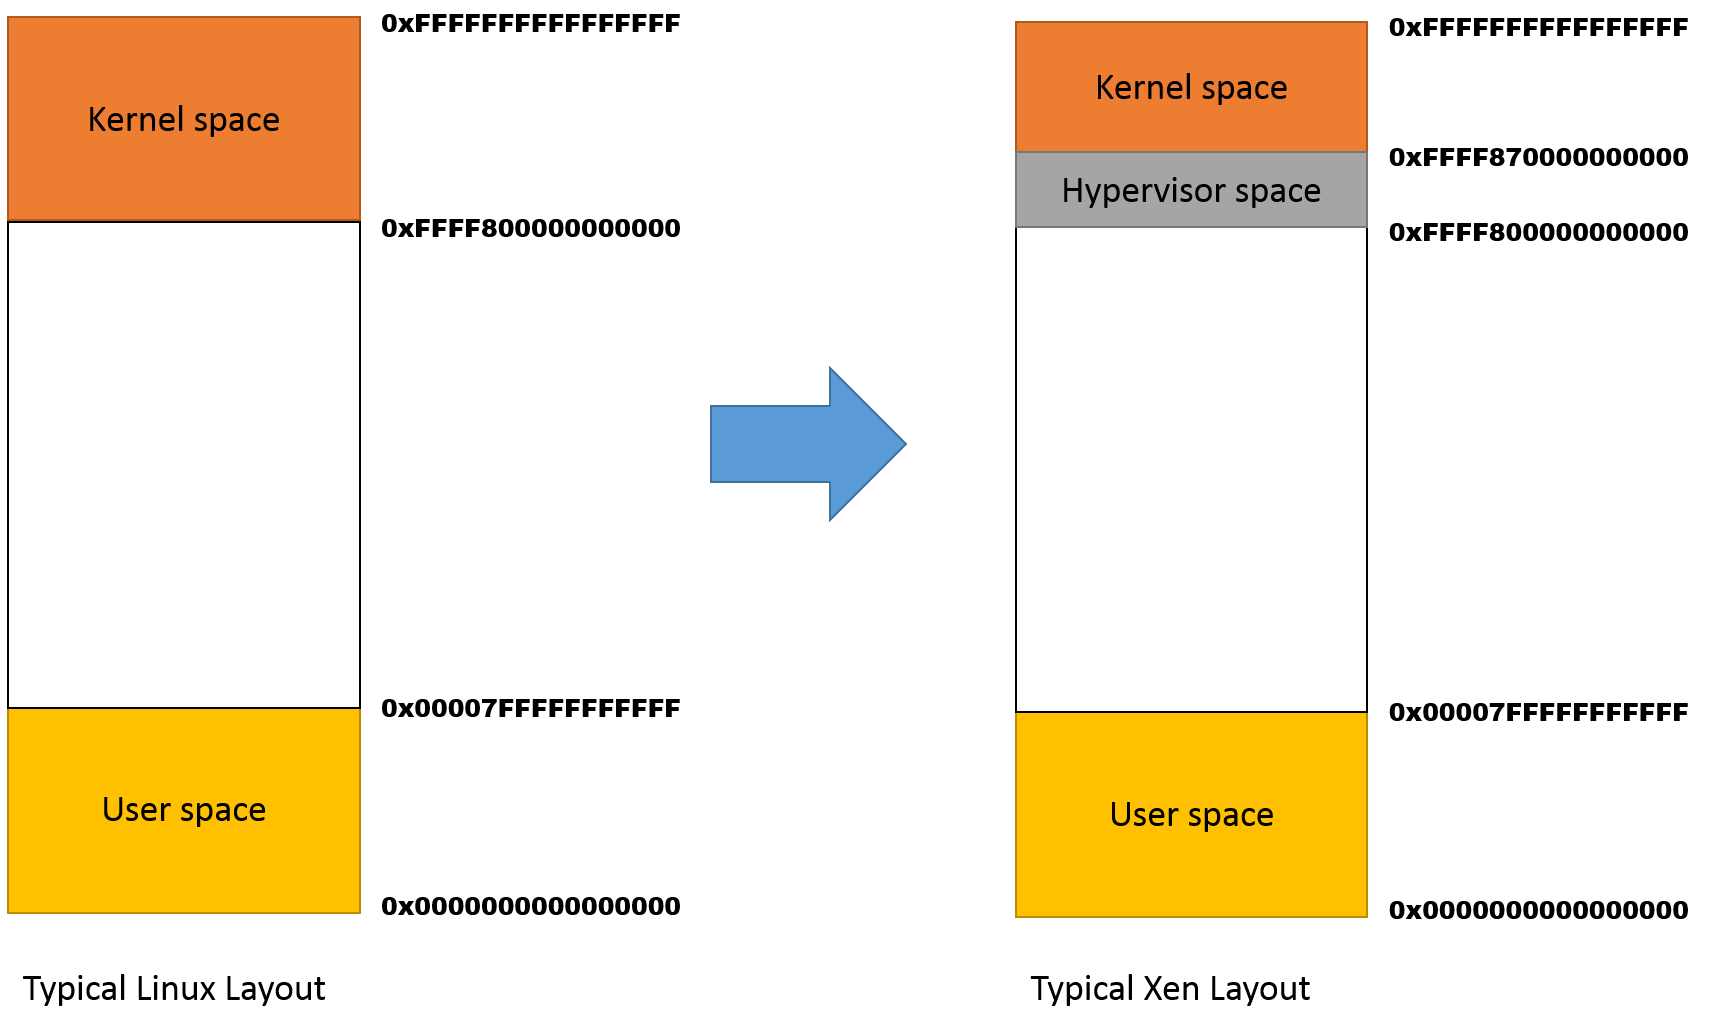
\includegraphics[scale=0.6]{figures/VA_layout_hypervisor.png}
\caption{Xen Virtual Address Layout Transformation}
\label{fig:xen_layout}
\end{figure}


A similar framework is setup in-between Xen hypervisor and the individual VMs (see Fig ~\ref{fig:xen_layout}). The hypervisor reserves a portion of the kernel address space for itself. This is done again to avoid context switches during hypercalls from a guest VM. This address space is again subdivided into different regions.. The memory layout is presented below: 



\begin{figure}[H]
\centering
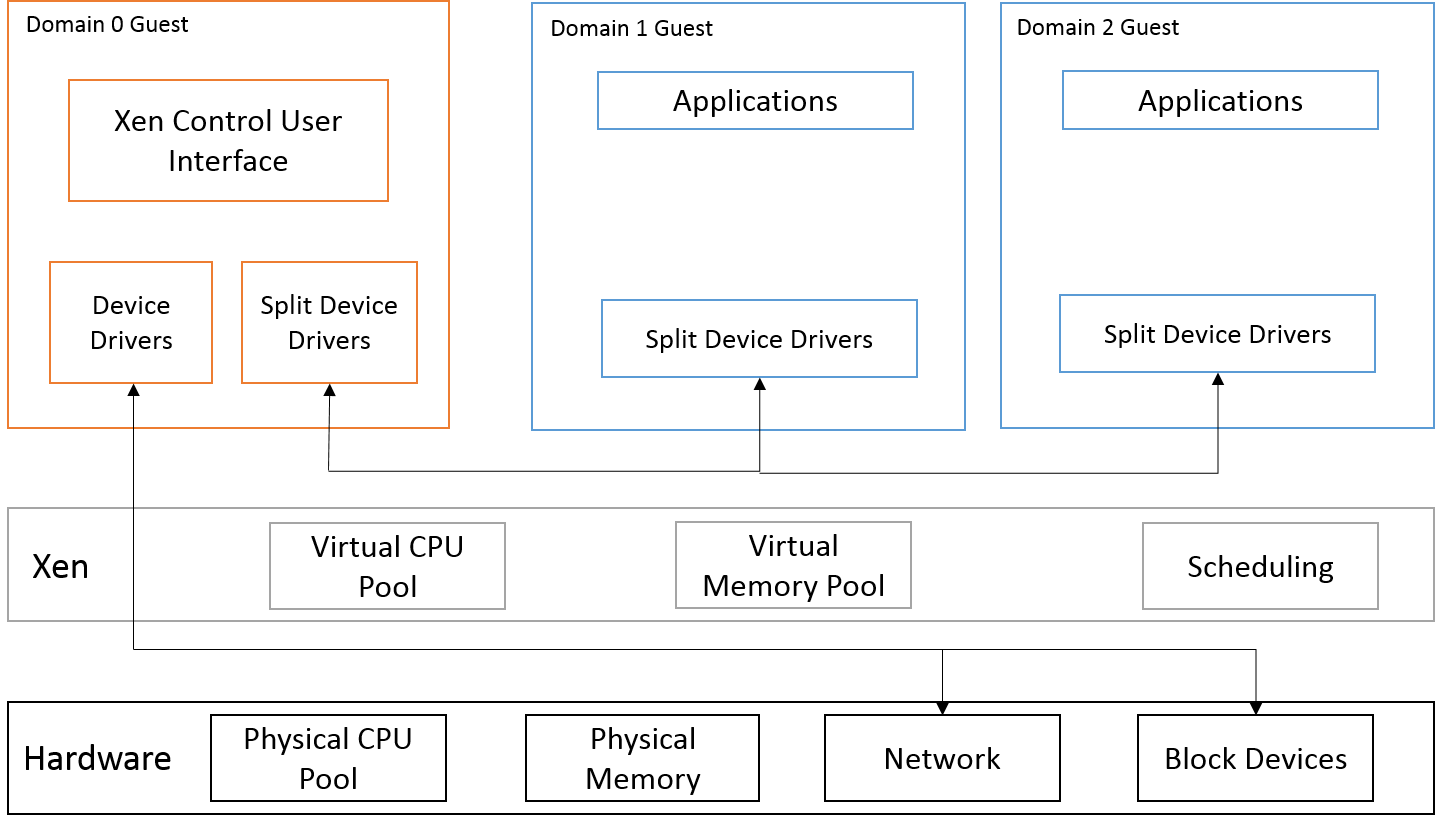
\includegraphics[scale=0.6]{figures/Xen_model.png}
\caption{Virtual Memory Regions}
\label{tab:xen_address}
\end{figure}

As seen in table ~\ref{tab:xen_address}, different regions, serve individual purposes, while the complete machine memory is made directly accessible to Xen through region 16. 


\subsection{Hypercalls}
Several hypercalls are provided to facilitate common memory management operations in Xen. Although in a pure virtualization environment, it is not necessary, but hypercalls are included for performance gains.  

 

Page table management is one of the most expensive operations in a paravirtualization approach. To prevent direct access to physical hardware, page tables of a domain are generally marked as read only by the hypervisor. Any attempted modifications by the guest VM would result in a trap to the VMM, which then emulates the required operation. 


Xen provides hypercalls for the guest to make the above procedure easier. It also allows for multiple page table changes to be clubbed together, via the HYPERVISOR\_mmu\_update hypercall. However, these operations are not relevant for the case of an HVM guest. In x86 architecture, the VT-x (for Intel chips) and SVM (for AMD chips) extensions allow the guest direct access to its own page tables. This eliminates the scenario for traps altogether.  

 

Thin provisioning is another important feature in a virtual machine. The balloon driver negotiates the actual memory occupied by a domain with the hypervisor. The popular commands used by it are XENMEM\_increase\_reservation, XENMEM\_decrease\_reservation and XENMEM\_populate\_physmap. The first two are used for runtime addition, or removal of memory blocks behind the guest physical address space. While the third one is used for the initial mapping of the guest address space during domain creation, for large memory requests. These commands are executed through the HYPERVISOR\_memory\_op hypercall. Another important command associated with this hypercall is XENMEM\_memory\_map. It can replace the BIOS call to provide an E820 memory map to a paravirtualized guest. Though not necessary for domU guests, it is one of the available ways to determine the initial layout of guest physical address space. 




\chapter{\uppercase{Design and Implementation}}

Conception of the proposed system revolves around the design of an additional memory management unit in the hypervisor. Since NVM data has existence beyond the lifetime of a VM, the conventional MMU cannot be used; its pages need a separate handler. A new Non-volatile memory management unit is presented as a solution, for a popular hypervisor -- Xen.  

In this chapter, several features of Xen are described relevant to the x86\_64 ISA with VT-x extensions and Intel Hub Architecture, followed by requisite modifications to incorporate the new MMU design. 

\section{Overview}

Boot procedure on x86 demands that the CPU should first transition from real mode to protected mode to access the entire address space. It should initialize the necessary page table data structure and segment registers to perform the switch, while keeping interrupts masked during the transition process. After entering the protected mode the processor has a lot more flexibility, but typically loses access to BIOS calls. For the above mentioned reasons, bootstrapping on x86 is a quite complex and tricky procedure. Typically, initialization of a MMU is one of the first tasks for any kernel, and it involves a fair amount of bootstrapping code. It makes this undertaking all the more challenging and interesting. This project can be broken down into two subdivisions. 

1. Create an independent Memory Management Unit for the available Non-Volatile RAM. 

2. Provide guest domains access to the NVRAM region, in a secure and protected manner. 

The first task requires modifications in the Xen kernel, with parts that deal with the boot process. Since the modifications are at the highest privilege level, it is very critical that the implementation be bug free, secure and efficient. Any blunders here could cause the entire system to crash.  

On the other hand, the second job deals more with user level code, specific to a toolchain. A notable part of domain creation focuses on emulation of firmware, performed mostly by various management tools. Only a small portion deals with issuing hypercalls resource allocation. Therefore, in this section most of the implementation details reside in the Xen control interface with minor modifications to the hypercall structure. Due to standardization of Xen API, a large number of tools have sprung up for VM management. This implementation picks up the xl toolchain, which currently is the default tool supported by Xen community. 

A basic outline of the implementation is presented below, with Fig. ~\ref{fig:xen_mod}, highlighting the modifications in red. 

1. Recognize the presence of NVRAM from E820 memory map provided by BIOS. 

2. Create a separate NVRAM pool to manage the resource independently. 

3. Create separate interface to specify DomU RAM and NVRAM requirements. 

4. Generate virtual E820 memory map reflecting NVRAM as a separate resource 

5. Map the virtual NVRAM space in domUs to the physical Non-volatile memory present on the machine. 

\begin{figure}[H]
\centering
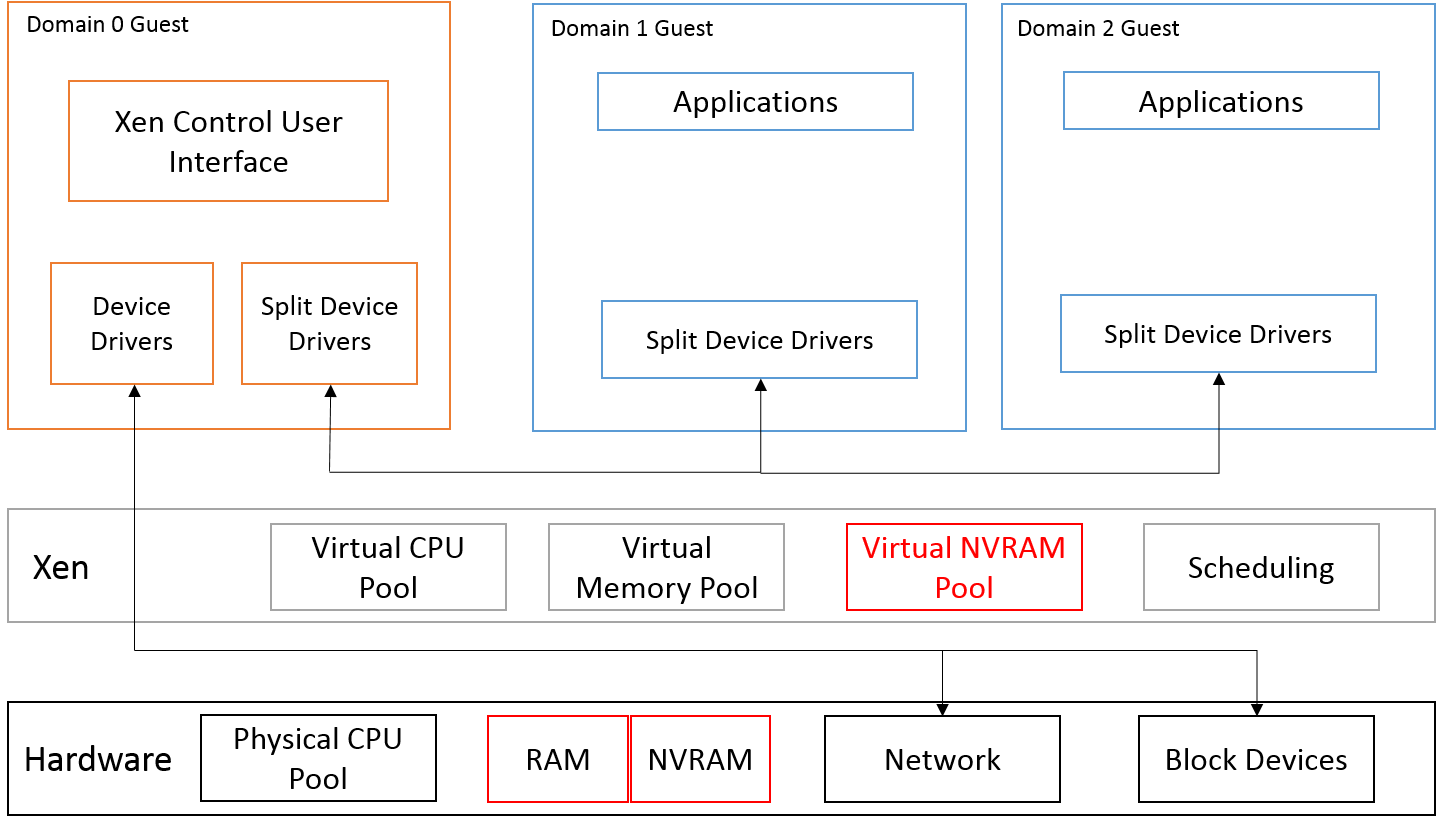
\includegraphics[scale=0.6]{figures/Xen_mod_model.png}
\caption{Modified Xen Architecture}
\label{fig:xen_mod}
\end{figure}

\section{Challenges}

There are several challenges faced during the design of the system in Xen. First and foremost is that current systems are not design for modular memory support. Xen has been architected around volatile memory banks, and the notion of a homogenous memory is integrated quite deep in the system design. This makes it all the more challenging to introduce another MMU. Moreover, major portion of the initialization is done during the boot procedure, which is in itself quite a complex process for x86. Along with the above virtualization being a relatively new technology lacks sufficient documentation. Thus even minor code changes turn into a grueling task. The combination of the above make the implementation an arduous but a stimulating and exciting challenge. 


\section{Xen Boot Procedure}

 

On system start, Xen boots up first to take stock of the hardware present. It queries the BIOS for the E820 Memory map. Identifying the available memory regions, Xen builds preliminary page tables and switches the machine to protected mode. With paging enabled, the hypervisor can access the entire address space. It follows by building the free page lists. Each machine page is identified by a data structure called page\_struct. This structure contains runtime administrative information about the machine page such as, status, domain identifier, special page status, order, etc. An array of these structures are initialized for all the machine pages. 

 

The next job is to build a buddy system allocator data structure arranging all the pages by MEMZONE and ORDER. Here MEMZONE divides the entire machine address space in terms of the position of the first non-zero bit. It is necessary for special DMA memory requests for devices with fewer address bits. In each ZONE the pages are sorted by the order of the contiguous available pages up to a maximum of 1GB. 

 

Memory requests are honored at page granularity by associated functions, which manipulate the above data structures following buddy system allocation. Pages returned by any domain are first scrubbed clean of all information and added to the pool, protecting the security across domains. The pool is always aggregated to the highest order on return requests. Direct mapping from a virtual address space to the machine addresses make these tasks a lot simpler. 

 

Once the memory pool is ready Domain 0 is given appropriate amount of memory and the kernel image is copied. The hypervisor follows to build a CPU pool out of the available cores. It initializes VMCS and other associated data structures and hands control over to Domain0 Linux kernel. It is the responsibility of dom0 now to initialize all I/O devices using their appropriate drivers. 

 

\section{Design modifications in Xen boot procedure}

To enable sharing NVRAM across separate VMs, we have to first recognize it as a memory region. Currently the firmware (BIOS) marks that section with code 90. Due to lack of standardization, this code is subject to change and presently not recognized by Xen. The hypervisor, therefore treats it as an unrecognized address space. Xen inhibits from either writing to, or reading from these addresses. 

 

The first task would be to recognize the memory region, and mark it as Non-Volatile RAM. A separate code word is added to the list of recognized E820 codes, to that effect. After identifying the region, a new NV memory manager along with associated NV memory pool is initialized. The E820 entries are examined one by one and the appropriate memory pools are populated, i.e. volatile RAM pool (identified by structure \_heap) is filled with RAM pages and non-volatile memory pool (identified by structure \_nvm\_heap) is filled with NVRAM pages. 

 

Once the memory pools are initialized, associated allocation functions can satisfy memory requests at page granularity. These functions just manipulate the memory pool data structures \_heap, \_nvm\_heap and page\_struct to mark the changes, without creating any additional page table mappings. Since all pages are accessible via direct mapping and Xen does not perform swapping, page table modifications are not needed. If the need arises, wrapper functions can be used in place. The structure page\_struct, which contains basic details for every page is also modified to add a flag marking the corresponding page as either volatile or non-volatile.  

 

With the above mentioned modifications in place Xen is able to boot up, identify the available Non-volatile memory and allocate/de-allocate NVRAM pages on demand. The following section uses this added functionality to dynamically allocate and map those pages to a domain. 

 

\section{Guest VM boot procedure}

Booting on bare metal x86 can be quite different from the virtual environment provided by Xen. An x86 CPU starts in 16 bit real mode, with BIOS providing basic essential functions such as hardware information, address space resolution and I/O device drivers. During the boot up procedure, the OS builds page tables and transitions the CPU to protected mode. At this point generally BIOS interrupt calls are unavailable so the OS device drivers are used for I/O. Most of the above functionalities are unavailable in a VM in Xen, because the hypervisor boots up first transitioning the machine into protected mode. This poses a problem as the CPU state is totally different in a VM to what an Operating System is expecting. 

 

A guest in Xen can boot in two available modes – PV and HVM. Both of them solve the above issue in separate ways. In PV mode the OS kernel is modified to allow booting in protected mode. Due to unavailability of BIOS, boot time information is passed to the guest using shared memory pages. There are two types of shared memory pages. 

1. Start info page: This page is mapped to the guest’s address space by Xen. It provides necessary information such as total available memory, number of virtual CPUs, console connection, and data structures regarding Xenstore. For boot purposes, Xen explicitly provides only a console device. Any other device must be mapped by the guest kernel using Xenstore services.  

2. Shared info pages: A guest kernel needs to explicitly map this page to its own address space for accessing dynamic runtime information about the virtual machine such as wall clock time, architectural information and event channels. This data is continually updated to reflect the status of the virtual machine. 

 

Information provided through these channels help in replacing BIOS functionality in PV guests. 

 

HVM mode, on the other hand, is supposed to run unmodified OSes, thus it has to forgo some of the performance benefits of the PV mode and emulate certain devices. Emulation is not optimal, because every abstract action is first converted to device specific commands by the guest OS device driver, and these commands are intercepted by Xen. The device emulator reconverts these device specific commands back to the abstract actions which are forwarded to the actual device driver for completion. The Xen split device driver model in PV guests generally run at a higher level of abstraction avoiding most of the redundant work observed above. 

 

BIOS is emulated by borrowing code from Bochs emulator. It forms the front end in a split device driver model, with the back end handled by code borrowed from QEMU, which is used to emulate devices in HVM mode. Xen starts a domain from the BIOS start point in the virtual 8086 mode present in x86. This mode is actually intended for running legacy application in real mode, alongside protected mode applications. Since it was designed for userspace code, the boot code of an OS (containing a good amount of sensitive instructions) result in numerous traps which have to be handled individually by Xen. 

 

In a hybrid approach Paravirtualized guests can take the benefit of paravirtualization techniques as well as hardware accelerators while running in HVM mode. The guest can specify a location in its ELF header where the hypercall page can be loaded. It can also execute the CPUID instruction to determine whether it is running on top of Xen or bare metal hardware. If running on Xen, the guest can choose to switch over to Xen specific device drivers, and also map the hypercall page during runtime. However, all these functions are typically performed after the kernel boots up, thus BIOS and QEMU emulator are generally needed during boot-up. 

 

Starting a domain begins with first defining a configuration file declaring the disk storage, memory, vCPU and other parameters. The command xl create <filename> performs certain administrative tasks in the userspace domain and then fires up the domain. Initially the xl tool parses the configuration file to identify resource requirements, most important of them being memory. If sufficient memory is not available, then an attempt is made to free up memory by communicating to Xen the additional memory requirement via Xenstore. This would typically result in Xen inflating the balloon drivers. In the event of still not meeting the memory requirement, the xl tool aborts the domain creation process with an error.  

 

On the other hand, if the memory requirements are met, the tool issues a hypercall (via xend) to build necessary data structures (VMCS and internal Xen data structures) for domain management. The management tool also creates a guest physical address space and sends a hypercall for appropriate memory allocation and page-table mappings. The hypervisor on receiving this hypercalls, allocates pages via the associated functions mentioned in the previous section. It also builds up the hypervisor page tables to map the guest physical pages to actual machine pages. If all is successful then a virtual E820 memory map is created, and the new VM is booted with emulated firmware using code borrowed from Bochs and QEMU.  

\section{Design modification}
The overall objective of this section is to create an interface for configuration and allocation of Non-volatile memory. Implementation details lie in three areas – xl management tool, Bochs emulator and hypercall structure. An interface is created initially for specifying the Non-volatile memory requirements in the domain config file. Once the requirements are specified, the tool chain creates additional guest physical address space for NVRAM. Actual memory allocation is performed at this point using hypercalls to notify the hypervisor of the guest physical page numbers with emphasis on allocation of contiguous memory blocks to minimize TLB entries. The x86\_64 architecture provides page mapping in the sizes of 1GB, 2MB and 4KB. The allocator moves in descending order for memory requests to satisfy the requirement. A flag is added to the hypercall argument to differentiate between volatile and non-volatile memory requests. If the flag is set, the hypervisor pulls pages out of the NVRAM pool, else it uses the RAM pool for the purpose. 

 

The above procedure completes one of the most critical portions of domain creation. Allocations of both volatile and non-volatile memory are complete and Xen is left with the task of firmware emulation. The toolchain creates virtual E820 table mappings, with an added region to indicate NVRAM with code 90. This completes the boot procedure and the virtual machine is equipped with non-volatile memory. When the VM is turned off, the hypervisor reclaims the NVRAM pages and adds them to the non-volatile memory pool.


